% Lecture 3 -- Stochastic integration: intuition, construction, applications
\documentclass[10pt,aspectratio=169]{beamer}

\usepackage[utf8]{inputenc}
\usepackage[T1]{fontenc}
\usepackage[english]{babel}
\usepackage{lmodern}
\usepackage{microtype}
\usepackage{amsmath,amssymb,bm,mathtools}
\usepackage{booktabs}
\usepackage{tikz}
\usetikzlibrary{arrows.meta,positioning,calc}

\usetheme[numbering=fraction,progressbar=frametitle]{metropolis}
\setbeamertemplate{frame numbering}[fraction]
\setbeamertemplate{navigation symbols}{}

\definecolor{BootcampBlueDark}{HTML}{1A3C68}
\definecolor{BootcampBlue}{RGB}{31,110,178}
\definecolor{AccentGold}{HTML}{DAA520}
\definecolor{SoftGray}{RGB}{245,246,248}
\definecolor{TextBlack}{HTML}{000000}
\definecolor{Crimson}{HTML}{990000}
\definecolor{MatrixGreen}{HTML}{228B22}

\setbeamercolor{normal text}{fg=TextBlack,bg=white}
\setbeamercolor{title}{fg=TextBlack}
\setbeamerfont{title}{size=\Large,series=\bfseries}
\setbeamercolor{structure}{fg=BootcampBlueDark}
\setbeamercolor{progress bar}{fg=BootcampBlueDark,bg=gray!30}
\setbeamercolor{frametitle}{bg=BootcampBlueDark,fg=white}
\setbeamerfont{frametitle}{series=\bfseries,size=\large}
\setbeamertemplate{frametitle}{
  \nointerlineskip
  \begin{beamercolorbox}[wd=\paperwidth,ht=3.2ex,dp=1.4ex,leftskip=1em,rightskip=1em]{frametitle}
    \usebeamerfont{frametitle}\insertframetitle
  \end{beamercolorbox}
}

\setbeamercolor{block title example}{bg=BootcampBlueDark!90!black,fg=white}
\setbeamercolor{block body example}{bg=BootcampBlueDark!5!white,fg=black}
\setbeamercolor{block title proposition}{bg=MatrixGreen!75!black,fg=white}
\setbeamercolor{block body proposition}{bg=MatrixGreen!7!white,fg=black}
\setbeamertemplate{blocks}[rounded][shadow=false]

\newenvironment{definitionblock}[1]{%
  \par\vspace{0.35em}%
  \begin{beamercolorbox}[wd=\textwidth,sep=0.35em,leftskip=0.3em,rightskip=0.6em]{block title example}%
    \raisebox{0.12em}{\usebeamerfont{block title example}#1}%
  \end{beamercolorbox}%
  \vspace{-0.35em}%
  \begin{beamercolorbox}[wd=\textwidth,sep=0.75em,leftskip=0.6em,rightskip=0.6em]{block body example}%
    \usebeamerfont{block body example}%
}{%
  \end{beamercolorbox}%
  \par\vspace{0.45em}%
}

\newenvironment{propositionblock}[1]{%
  \par\vspace{0.35em}%
  \begin{beamercolorbox}[wd=\textwidth,sep=0.35em,leftskip=0.3em,rightskip=0.6em]{block title proposition}%
    \raisebox{0.12em}{\usebeamerfont{block title example}#1}%
  \end{beamercolorbox}%
  \vspace{-0.35em}%
  \begin{beamercolorbox}[wd=\textwidth,sep=0.75em,leftskip=0.6em,rightskip=0.6em]{block body proposition}%
    \usebeamerfont{block body example}%
}{%
  \end{beamercolorbox}%
  \par\vspace{0.45em}%
}

\newcommand{\E}{\mathbb E}
\newcommand{\Pp}{\mathbb P}
\newcommand{\F}{\mathcal F}
\newcommand{\R}{\mathbb R}
\newcommand{\dd}{\,\mathrm d}
\newcommand{\Ito}{\mathrm{It\hat{o}}}
\DeclareMathOperator{\Var}{Var}
\DeclareMathOperator{\Cov}{Cov}

% One clean transition page per major section.
\AtBeginSection[]{
  \begin{frame}[plain]
    \vfill
    {\Large\bfseries\color{BootcampBlueDark}\insertsectionhead\par}
    \medskip
    {\color{BootcampBlueDark}\rule{0.9\textwidth}{0.8pt}}
    \vfill
  \end{frame}
}

\title{Stochastic Integration: Intuition, Construction, and Applications}
\author{}
\date{}

\begin{document}

\begin{frame}[plain]
  \vfill
  {\usebeamerfont{title}\usebeamercolor[fg]{title}\inserttitle\par}
  \medskip
  {\color{BootcampBlueDark}\rule{0.95\textwidth}{0.8pt}}
  \vfill
\end{frame}

\begin{frame}{References}
\footnotesize
\textbf{Main references}
\begin{itemize}\setlength{\itemsep}{0.55em}
  \item S.~Shreve, \emph{Stochastic Calculus for Finance II}, Chapter 4.
  \item I.~Karatzas and S.~Shreve, \emph{Brownian Motion and Stochastic Calculus}, Chapter 2.
  \item T.~Bj\"ork, \emph{Arbitrage Theory in Continuous Time}, chapter on stochastic integration.
\end{itemize}
\begin{block}{Scope of this lecture}
We build the \(\Ito\) integral just far enough to use it confidently. The \(\Ito\) formula comes in the next lecture.
\end{block}
\end{frame}

\begin{frame}{Roadmap}
\begin{enumerate}\setlength{\itemsep}{0.45em}
  \item Start from discrete trading gains and understand the left-point rule.
  \item Define the integral for simple predictable processes.
  \item Use the \(\Ito\) isometry to extend the definition.
  \item Check the integrability needed for a true martingale.
  \item Compute distributions and conditional laws in concrete examples.
  \item Compare left-, midpoint-, and right-point conventions.
  \item End with simulation rules and diagnostic checks.
\end{enumerate}
\end{frame}

% =====================================================
\section{Why Brownian Motion Needs a New Integral}
\subsection{Gains, roughness, and information}

\begin{frame}{A trading gain is a weighted sum of fresh price moves}
On a grid \(0=t_0<t_1<\cdots<t_n=T\), let \(\phi_{t_i}\) be the number of shares held during \((t_i,t_{i+1}]\).
The cumulative gain is
\[
G_T^\pi=\sum_{i=0}^{n-1}\phi_{t_i}\bigl(S_{t_{i+1}}-S_{t_i}\bigr).
\]
\begin{center}
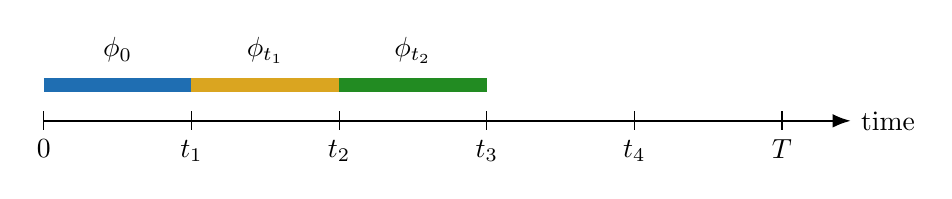
\begin{tikzpicture}[x=1.25cm,>=Latex]
  \draw[->,thick] (0,0)--(8.2,0) node[right] {time};
  \foreach \x/\lab in {0/0,1.5/t_1,3/t_2,4.5/t_3,6/t_4,7.5/T}
    \draw (\x,.12)--(\x,-.12) node[below] {\(\lab\)};
  \draw[line width=5pt,BootcampBlue] (0,.45)--(1.5,.45);
  \draw[line width=5pt,AccentGold] (1.5,.45)--(3,.45);
  \draw[line width=5pt,MatrixGreen] (3,.45)--(4.5,.45);
  \node at (.75,.9) {\(\phi_{0}\)};
  \node at (2.25,.9) {\(\phi_{t_1}\)};
  \node at (3.75,.9) {\(\phi_{t_2}\)};
\end{tikzpicture}
\end{center}
\begin{block}{Continuous-time target}
The stochastic integral should be the limit of these gains as the trading mesh becomes finer.
\end{block}
\end{frame}

\begin{frame}{Classical pathwise integration relies on smoothness or finite variation}
For differentiable paths, one may write
\[
\int_0^T \phi_t\dd S_t
=\int_0^T \phi_t S'_t\dd t.
\]
More generally, the Riemann--Stieltjes integral works well when the integrator has finite variation.
\begin{columns}[T,onlytextwidth]
\column{0.48\textwidth}
\begin{block}{Smooth path}
Small increments are essentially linear in \(\Delta t\), so their total variation remains controlled.
\end{block}
\column{0.48\textwidth}
\begin{block}{Brownian path}
\(\Delta W\) has typical size \(\sqrt{\Delta t}\). Total variation explodes as the mesh is refined.
\end{block}
\end{columns}
Brownian motion is continuous, but it is almost surely nowhere differentiable and of infinite variation.
\end{frame}

\begin{frame}{Quadratic variation is the scale that survives refinement}
For a partition \(\pi\) of \([0,T]\), define
\[
Q_T^\pi=\sum_i\bigl(W_{t_{i+1}}-W_{t_i}\bigr)^2.
\]
If the grid has \(n\) equal intervals, each square is typically of size \(T/n\), so the sum remains of order \(T\).
\begin{propositionblock}{Brownian quadratic variation}
As \(|\pi|\to0\),
\[
Q_T^\pi\longrightarrow T
\]
in probability, and along standard nested partitions almost surely.
\end{propositionblock}
This surviving second-order term is why ordinary calculus must be modified.
\end{frame}

\begin{frame}{The evaluation point changes the limiting answer}
Take the integrand \(\phi_t=W_t\). On the same partition, compare
\[
L^\pi=\sum_i W_{t_i}\Delta W_i,
\qquad
R^\pi=\sum_i W_{t_{i+1}}\Delta W_i.
\]
Since \(W_{t_{i+1}}=W_{t_i}+\Delta W_i\),
\[
R^\pi-L^\pi=\sum_i(\Delta W_i)^2\longrightarrow T.
\]
\begin{block}{Consequence}
There is no convention-free object called \(\int W\dd W\). The choice of sampling point matters by an order-one amount.
\end{block}
The \(\Ito\) integral uses left endpoints.
\end{frame}

\begin{frame}{Left endpoints are an information constraint, not a cosmetic choice}
At time \(t_i\), the trader knows \(\F_{t_i}\) and chooses \(\phi_{t_i}\) before observing \(\Delta S_i\).
\[
\underbrace{\phi_{t_i}}_{\F_{t_i}\text{-measurable}}
\times
\underbrace{(S_{t_{i+1}}-S_{t_i})}_{\text{future move}}.
\]
\begin{definitionblock}{Predictable in the discrete picture}
The position used over \((t_i,t_{i+1}]\) must be determined by information available at \(t_i\).
\end{definitionblock}
Using \(\phi_{t_{i+1}}\) would allow the strategy to react after seeing the move it is supposed to earn.
\begin{block}{Financial reading}
The \(\Ito\) convention encodes non-anticipative trading.
\end{block}
\end{frame}

\begin{frame}{Quick exercise: which trading rules are admissible?}
On the grid \(0,1,2\), let \(\Delta W_i=W_{i+1}-W_i\). Which positions are chosen without looking ahead?
\begin{enumerate}\setlength{\itemsep}{0.75em}
  \item \(\phi_0=1\), \(\phi_1=1+W_1^2\).
  \item \(\phi_0=\operatorname{sign}(W_1)\), \(\phi_1=0\).
  \item \(\phi_0=0\), \(\phi_1=\mathbf 1_{\{W_1>0\}}\).
  \item \(\phi_i=\operatorname{sign}(\Delta W_i)\).
\end{enumerate}
\begin{block}{Test}
For the position held on \((i,i+1]\), ask whether it is \(\F_i\)-measurable.
\end{block}
\end{frame}

\begin{frame}{Exercise debrief: admissibility is checked one interval at a time}
\begin{center}
\begin{tabular}{cll}
\toprule
Rule & Verdict & Reason \\
\midrule
1 & admissible & \(1+W_1^2\) is known at time \(1\) \\
2 & not admissible & \(W_1\) is unknown at time \(0\) \\
3 & admissible & the event \(\{W_1>0\}\) is in \(\F_1\) \\
4 & not admissible & \(\Delta W_i\) is the future move \\
\bottomrule
\end{tabular}
\end{center}
\begin{block}{Takeaway}
An integrand may be random and path-dependent. What matters is that it uses only the past and present, never the next increment.
\end{block}
\end{frame}

\begin{frame}{A predictable position cannot manufacture average drift}
Suppose \(S=W\) for the moment and \(\phi_{t_i}\in\F_{t_i}\). Then
\[
\E\bigl[\phi_{t_i}\Delta W_i\mid\F_{t_i}\bigr]
=\phi_{t_i}\E[\Delta W_i\mid\F_{t_i}]=0.
\]
Summing and taking expectations gives
\[
\E[G_T^\pi]=0.
\]
\begin{block}{Sanity check}
A non-anticipative strategy may change risk dramatically, but it cannot create a positive expected gain from a Brownian martingale.
\end{block}
This discrete identity will survive in the continuous-time integral.
\end{frame}

% =====================================================
\section{Build the Integral from Simple Strategies}
\subsection{Definition and first applications}

\begin{frame}{We integrate predictable processes with finite energy}
Let \((W_t)_{0\le t\le T}\) be Brownian motion with filtration \((\F_t)\).
The intended integrand \(\phi\) must satisfy two requirements:
\begin{enumerate}\setlength{\itemsep}{0.75em}
  \item \textbf{No anticipation:} \(\phi_t\) is predictable.
  \item \textbf{Finite energy:}
  \[
  \E\int_0^T\phi_t^2\dd t<\infty.
  \]
\end{enumerate}
\begin{block}{Why the square?}
Brownian increments have variance \(\Delta t\). This \(L^2\) condition controls the gain variance and later guarantees the \(L^1\) integrability required in the definition of a martingale.
\end{block}
We first define the integral for strategies that are constant between trading dates.
\end{frame}

\begin{frame}{Simple predictable processes are continuous-time trading rules}
Fix \(0=t_0<t_1<\cdots<t_n=T\). A simple predictable process has the form
\[
\phi_t=\sum_{i=0}^{n-1}\xi_i\mathbf 1_{(t_i,t_{i+1}]}(t),
\qquad \xi_i\in\F_{t_i}.
\]
\begin{center}
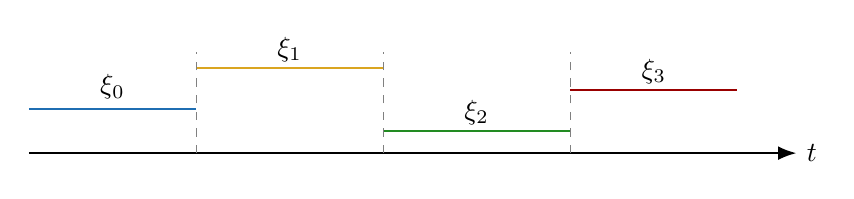
\begin{tikzpicture}[x=1.25cm,y=.8cm,>=Latex]
  \draw[->,thick] (0,0)--(7.8,0) node[right] {\(t\)};
  \draw[thick,BootcampBlue] (0,.7)--(1.7,.7);
  \draw[thick,AccentGold] (1.7,1.35)--(3.6,1.35);
  \draw[thick,MatrixGreen] (3.6,.35)--(5.5,.35);
  \draw[thick,Crimson] (5.5,1.0)--(7.2,1.0);
  \draw[dashed,gray] (1.7,0)--(1.7,1.6) (3.6,0)--(3.6,1.6) (5.5,0)--(5.5,1.6);
  \node at (.85,1.05) {\(\xi_0\)};
  \node at (2.65,1.65) {\(\xi_1\)};
  \node at (4.55,.65) {\(\xi_2\)};
  \node at (6.35,1.3) {\(\xi_3\)};
\end{tikzpicture}
\end{center}
The random coefficient \(\xi_i\) is chosen at \(t_i\) and held over the next interval.
\end{frame}

\begin{frame}{Definition: integrate a simple strategy by summing its gains}
\small
\begin{definitionblock}{\(\Ito\) integral of a simple predictable process}
For
\[
\phi_t=\sum_{i=0}^{n-1}\xi_i\mathbf 1_{(t_i,t_{i+1}]}(t),
\]
define
\[
\boxed{
\int_0^T\phi_t\dd W_t
:=\sum_{i=0}^{n-1}\xi_i\bigl(W_{t_{i+1}}-W_{t_i}\bigr).}
\]
\end{definitionblock}
This is exactly the discrete self-financing gain associated with the strategy \(\phi\).
\begin{block}{Units}
Position \(\times\) price move \(=\) gain. The notation records a limiting trading operation, not an ordinary product of \(\phi_t\), \(\dd W_t\), and \(\dd t\).
\end{block}
\end{frame}

\begin{frame}{Three sanity checks should become automatic}
For \(0\le a<b\le T\) and a constant \(c\),
\[
\int_0^T c\,\dd W_t=cW_T,
\]
\[
\int_0^T\mathbf 1_{(a,b]}(t)\dd W_t=W_b-W_a,
\]
and, for \(0<u<T\),
\[
\int_0^T\phi_t\dd W_t
=\int_0^u\phi_t\dd W_t+\int_u^T\phi_t\dd W_t.
\]
\begin{block}{Interpretation}
The integral adds the Brownian moves on the intervals where the position is active, weighted by the position held there.
\end{block}
\end{frame}

\begin{frame}{Worked example: a deterministic step strategy}
Let \(T=3\) and
\[
\phi_t=2\mathbf 1_{(0,1]}(t)-\mathbf 1_{(1,3]}(t).
\]
Then
\[
I=\int_0^3\phi_t\dd W_t
=2W_1-(W_3-W_1).
\]
The two increments are independent, so
\[
I\sim\mathcal N(0,4\cdot1+1\cdot2)
=\mathcal N(0,6).
\]
\begin{block}{Reading the variance}
Each interval contributes \((\text{position})^2\times(\text{length})\):
\(2^2\cdot1+(-1)^2\cdot2=6\).
\end{block}
\end{frame}

\begin{frame}{Exercise: switch the strategy after observing \(W_1\)}
Let \(A=\{W_1>0\}\) and define
\[
\phi_t=\mathbf 1_A\mathbf 1_{(1,2]}(t).
\]
\begin{block}{Your turn -- 3 minutes}
\begin{enumerate}\setlength{\itemsep}{0.5em}
  \item Explain why \(\phi\) is predictable.
  \item Write \(I=\int_0^2\phi_t\dd W_t\) without integral notation.
  \item Compute \(\E[I]\) and \(\E[I^2]\).
  \item Is \(I\) Gaussian?
\end{enumerate}
\end{block}
This example separates two ideas: the integrand is random, but the next increment remains fresh.
\end{frame}

\begin{frame}{Exercise debrief: a random integrand need not produce a Gaussian}
Because \(A\in\F_1\), the position is known before the interval \((1,2]\). By definition,
\[
I=\mathbf 1_A(W_2-W_1).
\]
The event \(A\) is independent of \(W_2-W_1\sim\mathcal N(0,1)\), hence
\[
\E[I]=0,
\qquad
\E[I^2]=\Pp(A)\E[(W_2-W_1)^2]=\tfrac12.
\]
But
\[
\Pp(I=0)=\Pp(A^c)=\tfrac12.
\]
\begin{block}{Conclusion}
The law is the mixture \(\frac12\delta_0+\frac12\mathcal N(0,1)\), not a Gaussian law. Gaussianity is automatic for deterministic integrands, not for arbitrary random ones.
\end{block}
\end{frame}

\begin{frame}{Linearity and time additivity mirror ordinary gains}
For simple predictable \(\phi,\psi\) and constants \(a,b\),
\[
\int_0^T(a\phi_t+b\psi_t)\dd W_t
=a\int_0^T\phi_t\dd W_t
+b\int_0^T\psi_t\dd W_t.
\]
For \(0\le s\le u\le t\),
\[
\int_s^t\phi_r\dd W_r
=\int_s^u\phi_r\dd W_r
+\int_u^t\phi_r\dd W_r.
\]
If \(\phi=\psi\) almost everywhere in \(\Omega\times[0,T]\), their integrals are the same almost surely.
\begin{block}{Practical message}
Split time into convenient pieces, simplify the integrand on each piece, and then add the gains.
\end{block}
\end{frame}

\begin{frame}{The integral up to time \(t\) is the accumulated gain process}
For a simple \(\phi\), define
\[
M_t=\int_0^t\phi_s\dd W_s.
\]
On an interval \((t_i,t_{i+1}]\),
\[
M_t=M_{t_i}+\xi_i(W_t-W_{t_i}).
\]
\begin{center}
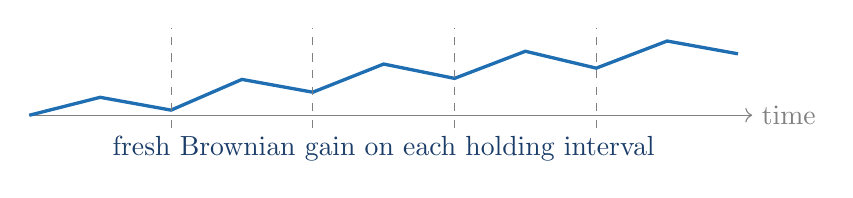
\begin{tikzpicture}[x=.9cm,y=.65cm]
  \draw[->,gray] (0,0)--(10.2,0) node[right] {time};
  \draw[very thick,BootcampBlue] plot coordinates
    {(0,0)(1,.35)(2,.1)(3,.7)(4,.45)(5,1.0)(6,.72)(7,1.25)(8,.92)(9,1.45)(10,1.2)};
  \foreach \x in {2,4,6,8} \draw[dashed,gray] (\x,-.25)--(\x,1.7);
  \node[BootcampBlueDark] at (5,-.65) {fresh Brownian gain on each holding interval};
\end{tikzpicture}
\end{center}
The continuous-time integral will preserve this interpretation after approximation.
\end{frame}

% =====================================================
\section{The Ito Isometry Does the Construction}
\subsection{Variance as integrand energy}

\begin{frame}{Disjoint Brownian increments are orthogonal}
Let \(\Delta W_i=W_{t_{i+1}}-W_{t_i}\). For \(i\neq j\),
\[
\E[\Delta W_i\Delta W_j]=0,
\]
while
\[
\E[(\Delta W_i)^2]=t_{i+1}-t_i.
\]
For predictable random coefficients, the useful conditional form is
\[
\E[\xi_i\Delta W_i\mid\F_{t_i}]=0.
\]
\begin{block}{Why cross terms disappear}
When the later increment is averaged conditional on everything known before it, its conditional mean is zero.
\end{block}
This is the stochastic analogue of orthogonality of perpendicular vectors.
\end{frame}

\begin{frame}{The Ito isometry converts variance into a time integral}
\small
\begin{propositionblock}{\(\Ito\) isometry for simple predictable processes}
If \(\phi\) is simple and predictable, then
\[
\boxed{
\E\left[\left(\int_0^T\phi_t\dd W_t\right)^2\right]
=\E\int_0^T\phi_t^2\dd t.}
\]
\end{propositionblock}
In norm notation,
\[
\left\|\int_0^T\phi_t\dd W_t\right\|_{L^2(\Omega)}
=\|\phi\|_{L^2(\Omega\times[0,T])}.
\]
\begin{block}{Meaning}
The map \(\phi\mapsto\int\phi\dd W\) preserves squared length. That is exactly the stability needed to take limits.
\end{block}
\end{frame}

\begin{frame}{The proof is one diagonal calculation}
Write \(I=\sum_i\xi_i\Delta W_i\). Then
\[
\E[I^2]
=\sum_i\E[\xi_i^2(\Delta W_i)^2]
+2\sum_{i<j}\E[\xi_i\Delta W_i\,\xi_j\Delta W_j].
\]
For \(i<j\), condition on \(\F_{t_j}\): the second factor \(\Delta W_j\) has conditional mean zero, so the cross term vanishes. On the diagonal,
\[
\E[\xi_i^2(\Delta W_i)^2]
=\E[\xi_i^2](t_{i+1}-t_i).
\]
Therefore
\[
\E[I^2]=\sum_i\E[\xi_i^2](t_{i+1}-t_i)
=\E\int_0^T\phi_t^2\dd t.
\]
\end{frame}

\begin{frame}{Mean and covariance come from the same computation}
For simple predictable \(\phi,\psi\),
\[
\E\left[\int_0^T\phi_t\dd W_t\right]=0
\]
and, by polarization,
\[
\boxed{
\E\left[
\left(\int_0^T\phi_t\dd W_t\right)
\left(\int_0^T\psi_t\dd W_t\right)
\right]
=\E\int_0^T\phi_t\psi_t\dd t.}
\]
\begin{block}{Orthogonality criterion}
If \(\phi_t\psi_t=0\) almost everywhere, the two integrals are uncorrelated. For deterministic integrands they are jointly Gaussian, hence independent.
\end{block}
\end{frame}

\begin{frame}{Energy of the strategy equals variance of the gain}
Define the pathwise exposure budget and its average energy by
\[
\mathcal E_T(\phi)=\int_0^T\phi_t^2\dd t,
\qquad
\E[\mathcal E_T(\phi)]=\E\int_0^T\phi_t^2\dd t.
\]
\begin{itemize}\setlength{\itemsep}{0.55em}
  \item Doubling \(\phi\) multiplies gain variance by \(4\).
  \item Holding the same position twice as long doubles variance.
  \item Moving exposure across time can preserve terminal variance while changing the gain path.
\end{itemize}
\begin{propositionblock}{A simple risk bound}
If \(|\phi_t|\le L\), then
\[
\Var\left(\int_0^T\phi_t\dd W_t\right)\le L^2T.
\]
\end{propositionblock}
\end{frame}

\begin{frame}{Exercise: two strategies with the same terminal risk}
On \([0,1]\), compare
\[
\phi_t=1,
\qquad
\psi_t=\sqrt2\,\mathbf 1_{(0,1/2]}(t).
\]
\begin{block}{Your turn -- 2 minutes}
\begin{enumerate}\setlength{\itemsep}{0.55em}
  \item Compute the energy of each strategy.
  \item Identify the two stochastic integrals.
  \item Compare their terminal distributions.
  \item Are the gain processes identical before time \(1\)?
\end{enumerate}
\end{block}
The isometry compares terminal risk, not the timing of that risk.
\end{frame}

\begin{frame}{Exercise debrief: equal energy gives equal Gaussian laws here}
Both deterministic strategies have unit energy:
\[
\int_0^1\phi_t^2\dd t=1,
\qquad
\int_0^1\psi_t^2\dd t=2\cdot\tfrac12=1.
\]
Their gains are
\[
\int_0^1\phi_t\dd W_t=W_1,
\qquad
\int_0^1\psi_t\dd W_t=\sqrt2\,W_{1/2}.
\]
Thus both are \(\mathcal N(0,1)\).
\begin{block}{But the paths differ}
The second strategy stops accumulating risk after time \(1/2\); the first remains exposed until time \(1\). Same terminal distribution does not mean same gain process.
\end{block}
\end{frame}

\begin{frame}{The completion idea is the entire extension argument}
Suppose simple predictable processes \(\phi^n\) approximate \(\phi\) so that
\[
\E\int_0^T|\phi_t^n-\phi_t|^2\dd t\longrightarrow0.
\]
By the isometry,
\[
\E\left[
\left|\int_0^T\phi_t^n\dd W_t-
\int_0^T\phi_t^m\dd W_t\right|^2
\right]
=\E\int_0^T|\phi_t^n-\phi_t^m|^2\dd t.
\]
The integrals are therefore Cauchy in \(L^2(\Omega)\), a complete space.
\begin{block}{Construction in one sentence}
Approximate the strategy, integrate the simple approximations, and take the \(L^2\) limit.
\end{block}
\end{frame}

\begin{frame}{Definition for a general square-integrable predictable integrand}
Let \(\phi\) be predictable with
\[
\E\int_0^T\phi_t^2\dd t<\infty.
\]
Choose simple predictable \(\phi^n\) converging to \(\phi\) in \(L^2(\Omega\times[0,T])\).
\begin{definitionblock}{General \(\Ito\) integral}
\[
\boxed{
\int_0^T\phi_t\dd W_t
:=L^2\text{-}\lim_{n\to\infty}
\int_0^T\phi_t^n\dd W_t.}
\]
\end{definitionblock}
The isometry shows that the limit exists and is independent of the chosen approximation. Linearity, mean zero, and the isometry pass to the limit.
\end{frame}

% =====================================================
\section{The Integral Is a Martingale Gain Process}
\subsection{Conditional applications}

\begin{frame}{Before saying ``martingale,'' check integrability}
Let \(\phi\) be predictable and assume, for every finite \(T\),
\[
\E\int_0^T\phi_s^2\dd s<\infty.
\]
Then, for \(M_t=\int_0^t\phi_s\dd W_s\), the isometry and Cauchy--Schwarz give
\[
\E|M_t|
\le \bigl(\E[M_t^2]\bigr)^{1/2}
=\left(\E\int_0^t\phi_s^2\dd s\right)^{1/2}<\infty.
\]
Thus \(M_t\in L^2\subset L^1\): its conditional expectation is well defined.
\begin{alertblock}{Do not confuse two levels of assumptions}
If only \(\int_0^T\phi_s^2\dd s<\infty\) almost surely, the integral is generally a \emph{local} martingale. The expectation condition above gives the square-integrable, hence true, martingale used here.
\end{alertblock}
\end{frame}

\begin{frame}{Finite expected energy gives a true martingale}
\small
For a predictable \(\phi\) satisfying
\[
\E\int_0^T\phi_s^2\dd s<\infty,
\qquad
M_t=\int_0^t\phi_s\dd W_s,
\]
\begin{propositionblock}{Square-integrable martingale property}
The process \(M\) is adapted, \(M_t\in L^2\), and, for \(0\le s\le t\le T\),
\[
\boxed{\E[M_t\mid\F_s]=M_s.}
\]
Equivalently,
\[
\E\left[\int_s^t\phi_u\dd W_u\middle|\F_s\right]=0.
\]
\end{propositionblock}
The future gain may have state-dependent risk, but its conditional mean is zero.
\end{frame}

\begin{frame}{The martingale proof repeats the discrete no-drift argument}
For a simple process on a grid containing \(s\), split
\[
M_t=M_s+\sum_{t_i\ge s}\xi_i\Delta W_i.
\]
For each future increment,
\[
\E[\xi_i\Delta W_i\mid\F_{t_i}]
=\xi_i\E[\Delta W_i\mid\F_{t_i}]=0.
\]
Iterated conditioning gives
\[
\E[M_t-M_s\mid\F_s]=0.
\]
The general case follows by \(L^2\) approximation. Since \(L^2\) convergence implies \(L^1\) convergence, conditional expectations pass to the limit.
\begin{block}{Proof pattern to remember}
Predictable coefficient \(\times\) fresh centered increment \(\Rightarrow\) zero conditional mean.
\end{block}
\end{frame}

\begin{frame}{Conditional variance measures the risk still ahead}
The conditional version of the isometry gives
\[
\boxed{
\E\left[
\left(\int_s^t\phi_u\dd W_u\right)^2
\middle|\F_s\right]
=\E\left[\int_s^t\phi_u^2\dd u\middle|\F_s\right].}
\]
\begin{columns}[T,onlytextwidth]
\column{0.48\textwidth}
\begin{block}{Conditional mean}
The future stochastic gain is zero on average given current information.
\end{block}
\column{0.48\textwidth}
\begin{block}{Conditional variance}
Current information can change how much future variance the strategy will accumulate.
\end{block}
\end{columns}
This distinction is central in hedging: no predictable drift does not mean no risk.
\end{frame}

\begin{frame}{Exercise: a state-dependent position changes future variance}
On \([0,2]\), define
\[
\phi_t=\mathbf 1_{(0,1]}(t)
+\bigl(1+\mathbf 1_{\{W_1>0\}}\bigr)\mathbf 1_{(1,2]}(t),
\qquad
M_t=\int_0^t\phi_s\dd W_s.
\]
\begin{block}{Your turn -- 3 minutes}
Compute, in terms of \(W_1\),
\begin{enumerate}\setlength{\itemsep}{0.5em}
  \item \(M_1\);
  \item \(\E[M_2\mid\F_1]\);
  \item \(\Var(M_2-M_1\mid\F_1)\).
\end{enumerate}
\end{block}
The position doubles after time \(1\) precisely on the event \(\{W_1>0\}\).
\end{frame}

\begin{frame}{Exercise debrief: the forecast is unchanged, the risk is not}
Up to time \(1\), the position is one, so
\[
M_1=W_1.
\]
The martingale property yields
\[
\E[M_2\mid\F_1]=M_1=W_1.
\]
Over \((1,2]\), the position is already known at time \(1\), hence
\[
\Var(M_2-M_1\mid\F_1)
=\bigl(1+\mathbf 1_{\{W_1>0\}}\bigr)^2
=\begin{cases}
1,&W_1\le0,\\
4,&W_1>0.
\end{cases}
\]
\begin{block}{Takeaway}
Adaptation can make future variance depend on the current state without creating conditional drift.
\end{block}
\end{frame}

\begin{frame}{Quadratic variation is the integral's variance clock}
For
\[
M_t=\int_0^t\phi_s\dd W_s,
\]
the quadratic variation satisfies
\[
\boxed{[M]_t=\int_0^t\phi_s^2\dd s.}
\]
For a simple strategy, this is suggested directly by
\[
\sum_i(\Delta M_i)^2
=\sum_i\xi_i^2(\Delta W_i)^2
\approx\sum_i\xi_i^2\Delta t_i.
\]
\begin{block}{Interpretation}
Calendar time runs at unit speed for \(W\). The gain process runs on the random clock generated by squared exposure.
\end{block}
\end{frame}

\begin{frame}{Stopping a strategy means switching the integrand off}
\small
Let \(\tau\) be a stopping time. Switching the position off at \(\tau\) gives
\[
\boxed{
\int_0^t\mathbf 1_{\{s\le\tau\}}\dd W_s
=W_{t\wedge\tau}.}
\]
For each finite \(t\), the stopped integrand is square-integrable because
\[
\E\int_0^t\mathbf 1_{\{s\le\tau\}}^2\dd s
=\E[t\wedge\tau]\le t.
\]
The martingale property and the isometry therefore apply:
\[
\boxed{
\E[W_{t\wedge\tau}]=0,
\qquad
\E[W_{t\wedge\tau}^2]=\E[t\wedge\tau].}
\]
This check is what licenses the two expectation identities; stopping alone is not a substitute for integrability.
\end{frame}

\begin{frame}{Application: stop Brownian exposure at a barrier}
Let \(\tau_a=\inf\{t\ge0:W_t=a\}\), with \(a>0\). The stopped exposure
\[
M_t=\int_0^t\mathbf 1_{\{s\le\tau_a\}}\dd W_s
=W_{t\wedge\tau_a}
\]
never continues after the upper barrier is reached.
\begin{block}{Your turn}
Use only the martingale property and isometry to identify
\[
\E[M_t]
\qquad\text{and}\qquad
\E[M_t^2].
\]
\end{block}
\begin{block}{Answer}
\[
\E[M_t]=0,
\qquad
\E[M_t^2]=\E[t\wedge\tau_a].
\]
\end{block}
No density of \(\tau_a\) is needed.
\end{frame}

\begin{frame}{Predictable Brownian trading transforms risk, not drift}
For every predictable strategy satisfying \(\E\int_0^T\phi_t^2\dd t<\infty\),
\[
\E\left[\int_0^T\phi_t\dd W_t\right]=0.
\]
Yet the distribution can be:
\begin{itemize}\setlength{\itemsep}{0.55em}
  \item Gaussian when \(\phi\) is deterministic;
  \item a non-Gaussian mixture when \(\phi\) reacts to past states;
  \item stopped, skewed, or state-dependent for more complex strategies.
\end{itemize}
\begin{block}{What remains invariant}
The gain process is a square-integrable martingale and its second moment is exactly the expected integrand energy.
\end{block}
This is the structural content of stochastic integration before any \(\Ito\) formula is used.
\end{frame}

% =====================================================
\section{Deterministic Integrands Give Explicit Gaussian Applications}
\subsection{Laws, covariance, and conditioning}

\begin{frame}{A deterministic integrand produces a Gaussian random variable}
Let \(f\in L^2(0,T)\) be deterministic. Then
\[
I_f=\int_0^T f(t)\dd W_t
\]
is a limit of Gaussian linear combinations of Brownian increments.
\begin{propositionblock}{Distribution}
\[
\boxed{
I_f\sim\mathcal N\!\left(0,\int_0^T f(t)^2\dd t\right).}
\]
\end{propositionblock}
The mean is zero and the variance comes from the isometry.
\begin{block}{Why the Gaussian law survives the limit}
The characteristic functions converge to that of the centered Gaussian with the limiting variance.
\end{block}
\end{frame}

\begin{frame}{Inner products of functions become covariances of integrals}
For deterministic \(f,g\in L^2(0,T)\),
\[
\Cov\left(\int_0^T f\dd W,\int_0^T g\dd W\right)
=\int_0^T f(t)g(t)\dd t.
\]
Moreover, the pair is jointly Gaussian.
\begin{propositionblock}{Independence criterion}
If
\[
\int_0^T f(t)g(t)\dd t=0,
\]
then \(\int f\dd W\) and \(\int g\dd W\) are independent.
\end{propositionblock}
Orthogonal deterministic exposure profiles generate independent Gaussian risks.
\end{frame}

\begin{frame}{Worked application: a linearly increasing exposure}
Take \(f(t)=t\). Then
\[
I_T=\int_0^T t\dd W_t
\]
is centered Gaussian with
\[
\Var(I_T)=\int_0^T t^2\dd t=\frac{T^3}{3}.
\]
Therefore
\[
\boxed{I_T\sim\mathcal N\!\left(0,\frac{T^3}{3}\right).}
\]
\begin{block}{Scaling check}
Brownian noise contributes \(\sqrt{\dd t}\), while the position grows like \(t\). The resulting standard deviation scales like \(T^{3/2}\).
\end{block}
\end{frame}

\begin{frame}{Exercise: condition an integral on the terminal Brownian value}
Let
\[
I_T=\int_0^T t\dd W_t.
\]
\begin{block}{Your turn -- 4 minutes}
\begin{enumerate}\setlength{\itemsep}{0.55em}
  \item Write \(W_T\) as a stochastic integral.
  \item Compute \(\Cov(I_T,W_T)\).
  \item Use Gaussian regression to find \(\E[I_T\mid W_T]\).
  \item Compute \(\Var(I_T\mid W_T)\).
\end{enumerate}
\end{block}
Recall that for a centered Gaussian pair \((X,Y)\),
\[
\E[X\mid Y]=\frac{\Cov(X,Y)}{\Var(Y)}Y.
\]
\end{frame}

\begin{frame}{Exercise debrief: conditioning is projection in function space}
Since
\[
W_T=\int_0^T1\dd W_t,
\]
the covariance formula gives
\[
\Cov(I_T,W_T)=\int_0^T t\dd t=\frac{T^2}{2}.
\]
Because \(\Var(W_T)=T\),
\[
\boxed{\E[I_T\mid W_T]=\frac{T}{2}W_T.}
\]
The residual conditional variance is
\[
\Var(I_T\mid W_T)
=\frac{T^3}{3}-\frac{(T^2/2)^2}{T}
=\frac{T^3}{12}.
\]
Only the component of the function \(t\mapsto t\) parallel to the constant function is revealed by \(W_T\).
\end{frame}

\begin{frame}{Exercise: construct a Gaussian risk independent of \(W_T\)}
We seek a nonzero deterministic \(g\) such that
\[
Y=\int_0^T g(t)\dd W_t
\]
is independent of \(W_T\).
\begin{block}{Your turn -- 2 minutes}
\begin{enumerate}\setlength{\itemsep}{0.55em}
  \item Translate independence into an integral condition on \(g\).
  \item Find a simple affine function \(g(t)=t-c\) satisfying it.
  \item Compute \(\Var(Y)\).
\end{enumerate}
\end{block}
The problem is ordinary orthogonality in \(L^2(0,T)\).
\end{frame}

\begin{frame}{Exercise debrief: center the exposure profile}
\small
Independence from \(W_T=\int_0^T1\dd W_t\) requires
\[
\int_0^T g(t)\dd t=0.
\]
Choose
\[
g(t)=t-\frac{T}{2}.
\]
Then
\[
\Cov(Y,W_T)=0,
\]
and joint Gaussianity gives \(Y\perp\!\!\!\perp W_T\). Its variance is
\[
\Var(Y)=\int_0^T\left(t-\frac{T}{2}\right)^2\dd t
=\frac{T^3}{12}.
\]
\begin{block}{Geometric reading}
Subtracting the average removes the component aligned with the terminal Brownian shock.
\end{block}
\end{frame}

\begin{frame}{Deterministic integrands create time-changed Brownian motions}
Define
\[
M_t=\int_0^t f(s)\dd W_s,
\qquad
q(t)=\int_0^t f(s)^2\dd s.
\]
The process \(M\) is centered Gaussian, has independent increments, and
\[
\Var(M_t-M_s)=q(t)-q(s).
\]
\begin{propositionblock}{Time-change viewpoint}
\[
(M_t)_{t\ge0}\ \overset{\mathrm{law}}=\ (B_{q(t)})_{t\ge0}
\]
for a Brownian motion \(B\).
\end{propositionblock}
For \(f(t)=t\), the stochastic clock is \(q(t)=t^3/3\).
\end{frame}

\begin{frame}{Integration by parts with a deterministic integrand}
\small
\begin{block}{Sufficient regularity}
Assume that \(f:[0,T]\to\R\) is deterministic and \(C^1\). More generally, it is enough that \(f\) be absolutely continuous with \(f'\in L^2(0,T)\). Then \(f\in L^2(0,T)\), and both integrals below exist.
\end{block}
Discrete summation by parts gives, in the limit,
\[
f(T)W_T-f(0)W_0
=\int_0^T f(t)\dd W_t
+\int_0^T W_t f'(t)\dd t.
\]
Since \(W_0=0\),
\[
\boxed{
\int_0^T f(t)\dd W_t
=f(T)W_T-\int_0^T W_t f'(t)\dd t.}
\]
\begin{block}{No \(\Ito\) formula is needed}
The deterministic path has finite variation, so its quadratic covariation with \(W\) is zero: there is no correction term.
\end{block}
\end{frame}

\begin{frame}{Application: identify the law of the Brownian area}
Set
\[
A_T=\int_0^T W_t\dd t.
\]
Using integration by parts with \(f(t)=t\),
\[
A_T=TW_T-\int_0^T t\dd W_t.
\]
Thus \(A_T\) is Gaussian and centered. From the covariance calculations,
\[
\Var(A_T)
=T^2\Var(W_T)+\Var(I_T)-2T\Cov(W_T,I_T)
=\frac{T^3}{3}.
\]
Therefore
\[
\boxed{A_T\sim\mathcal N\!\left(0,\frac{T^3}{3}\right).}
\]
This path-dependent functional is handled without evaluating any density by hand.
\end{frame}

% =====================================================
\section{Left, Right, and Midpoint Conventions}
\subsection{The first Ito correction}

\begin{frame}{Three natural sums lead to three different limits}
For \(\phi_t=W_t\) and partition \(\pi\), define
\[
L^\pi=\sum_iW_{t_i}\Delta W_i,
\qquad
M^\pi=\sum_i\frac{W_{t_i}+W_{t_{i+1}}}{2}\Delta W_i,
\qquad
R^\pi=\sum_iW_{t_{i+1}}\Delta W_i.
\]
\begin{center}
\begin{tabular}{lll}
\toprule
Sum & Information & Limiting convention \\
\midrule
left & known before the move & \(\Ito\) \\
midpoint & uses both endpoints & Stratonovich \\
right & known after the move & anticipative here \\
\bottomrule
\end{tabular}
\end{center}
Brownian quadratic variation prevents these sums from collapsing to the same answer.
\end{frame}

\begin{frame}{An exact algebraic identity isolates the correction}
For every interval,
\[
W_{t_{i+1}}^2-W_{t_i}^2
=2W_{t_i}\Delta W_i+(\Delta W_i)^2.
\]
Summing over \(i\),
\[
W_T^2
=2L^\pi+\sum_i(\Delta W_i)^2.
\]
As the mesh tends to zero,
\[
\sum_i(\Delta W_i)^2\longrightarrow T.
\]
\begin{block}{This is the whole mechanism}
The square of a Brownian increment is small on one interval but accumulates to an order-one correction over many intervals.
\end{block}
\end{frame}

\begin{frame}{The first nontrivial stochastic integral can be computed directly}
Passing to the limit in the left-sum identity gives
\[
\boxed{
\int_0^T W_t\dd W_t
=\frac12\bigl(W_T^2-T\bigr).}
\]
Compare this with the classical formula \(\int x\dd x=\frac12x^2\).
\begin{block}{Ito correction}
The additional \(-T/2\) exactly compensates for Brownian quadratic variation and restores the zero-mean martingale property:
\[
\E\left[\frac12(W_T^2-T)\right]=0.
\]
\end{block}
No general \(\Ito\) formula was needed -- only a telescoping identity and \([W]_T=T\).
\end{frame}

\begin{frame}{Right and midpoint sums reveal the size of the convention effect}
Since
\[
R^\pi=L^\pi+\sum_i(\Delta W_i)^2,
\]
the right-point limit is
\[
\frac12(W_T^2-T)+T
=\frac12(W_T^2+T).
\]
The midpoint sum is the average of left and right sums, so its limit is
\[
\frac12W_T^2.
\]
\begin{center}
\begin{tabular}{lc}
\toprule
Convention & Limit for \(\int_0^T W\dd W\) \\
\midrule
left / \(\Ito\) & \(\frac12(W_T^2-T)\) \\
midpoint / Stratonovich & \(\frac12W_T^2\) \\
right & \(\frac12(W_T^2+T)\) \\
\bottomrule
\end{tabular}
\end{center}
\end{frame}

\begin{frame}{Exercise: verify the isometry on \(\int_0^T W_t\dd W_t\)}
Let
\[
I_T=\int_0^T W_t\dd W_t
=\frac12(W_T^2-T).
\]
\begin{block}{Your turn -- 3 minutes}
\begin{enumerate}\setlength{\itemsep}{0.55em}
  \item Compute \(\E[I_T]\).
  \item Using \(\E[W_T^4]=3T^2\), compute \(\E[I_T^2]\).
  \item Check that the result agrees with the \(\Ito\) isometry.
\end{enumerate}
\end{block}
This is a useful consistency test between the explicit formula and the abstract construction.
\end{frame}

\begin{frame}{Exercise debrief: the explicit formula matches the isometry}
Since \(\E[W_T^2]=T\),
\[
\E[I_T]=0.
\]
Moreover,
\[
\E[I_T^2]
=\frac14\E[(W_T^2-T)^2]
=\frac14(3T^2-2T^2+T^2)
=\frac{T^2}{2}.
\]
The isometry gives the same answer:
\[
\E\left[\left(\int_0^T W_t\dd W_t\right)^2\right]
=\E\int_0^T W_t^2\dd t
=\int_0^T t\dd t
=\frac{T^2}{2}.
\]
Two routes, one answer.
\end{frame}

\begin{frame}{Seeing the next increment would create a fake arbitrage}
Suppose illegally that the trader could choose
\[
\phi_{t_i}=\operatorname{sign}(\Delta W_i)
\]
before reporting the gain. Then
\[
\sum_i\phi_{t_i}\Delta W_i
=\sum_i|\Delta W_i|\ge0,
\]
and it is strictly positive with probability one on a nontrivial grid.
\begin{block}{What failed?}
The position is not \(\F_{t_i}\)-measurable: it uses the very move it claims to predict. This is not a trading strategy; it is hindsight.
\end{block}
Predictability is therefore both the mathematical and economic boundary of the \(\Ito\) integral.
\end{frame}

\subsection{Simulation and diagnostic checks}

\begin{frame}{Simulation means implementing the left-point rule}
\small
On the uniform grid \(t_i=i\Delta t\), with \(\Delta t=T/n\), generate
\[
Z_i\overset{\mathrm{iid}}{\sim}\mathcal N(0,1),
\qquad
\Delta W_i=\sqrt{\Delta t}\,Z_i.
\]
Starting from \(W_0=I_0=0\), repeat at each step:
\begin{enumerate}\setlength{\itemsep}{0.45em}
  \item compute \(\phi_i\) using only information available at \(t_i\);
  \item update \(I_{i+1}=I_i+\phi_i\Delta W_i\);
  \item update \(W_{t_{i+1}}=W_{t_i}+\Delta W_i\).
\end{enumerate}
Then
\[
I_n=\sum_{i=0}^{n-1}\phi_i\Delta W_i
\approx \int_0^T\phi_t\dd W_t.
\]
\begin{block}{The order is mathematical, not cosmetic}
If \(\phi_i\) uses \(W_{t_{i+1}}\) or the newly generated \(\Delta W_i\), the scheme is no longer a left-point \(\Ito\) sum.
\end{block}
\end{frame}

\begin{frame}{A theoretical benchmark for the simulation error}
\footnotesize
For the integral \(I=\int_0^T W_t\dd W_t\), simulate the left sum
\[
I^{(n)}=\sum_{i=0}^{n-1}W_{t_i}\Delta W_i.
\]
The exact identity \(I=\tfrac12(W_T^2-T)\) gives
\[
I-I^{(n)}
=\frac12\sum_{i=0}^{n-1}\bigl((\Delta W_i)^2-\Delta t\bigr).
\]
On a uniform grid, independence and
\(\Var((\Delta W_i)^2)=2(\Delta t)^2\) yield
\[
\boxed{\E\bigl[(I-I^{(n)})^2\bigr]=\frac{T^2}{2n}.}
\]
\begin{block}{A useful unit test}
The root-mean-square error should decay like \(n^{-1/2}\). This tests the simulation against a theorem, not a visually plausible path.
\end{block}
\end{frame}

\begin{frame}{Classic simulation traps and how to detect them}
\footnotesize
\begin{itemize}\setlength{\itemsep}{0.3em}
  \item \textbf{Wrong Brownian scale:} using \(\Delta t\,Z_i\) instead of \(\sqrt{\Delta t}\,Z_i\) destroys the variance clock.
  \item \textbf{Looking one step ahead:} computing \(\phi_i\) from \(W_{t_{i+1}}\) produces a right-point, anticipative sum and typically adds a bias.
  \item \textbf{Wrong noise coupling:} if the integrand and the integral are driven by the same Brownian motion, they must use the same increments; fresh independent noise changes their joint law.
  \item \textbf{Confusing \(\dd W\) and \(\dd t\):} \(\sum_i\phi_i\Delta W_i\) approximates a stochastic integral, while \(\sum_i\phi_i\Delta t\) approximates an ordinary time integral.
  \item \textbf{Checking only the mean:} also compare the empirical second moment with \(\E\int_0^T\phi_t^2\dd t\), and test several grid sizes.
\end{itemize}
\begin{alertblock}{Filtration check}
At every step, ask: was \(\phi_i\) fully determined before \(\Delta W_i\) was used?
\end{alertblock}
\end{frame}

\begin{frame}{What to retain before learning the Ito formula}
\small
\begin{enumerate}\setlength{\itemsep}{0.25em}
  \item \(\int\phi\dd W\) is the limit of left-point, non-anticipative gains built first for simple predictable strategies.
  \item The isometry converts integrand energy into gain variance and makes the \(L^2\) extension possible.
  \item Under \(\E\int_0^T\phi_t^2\dd t<\infty\), the integral process is a square-integrable martingale with quadratic variation \(\int\phi^2\dd t\).
  \item Deterministic integrands give explicit jointly Gaussian variables.
  \item Brownian quadratic variation creates the correction
  \[
  \int_0^T W_t\dd W_t=\tfrac12(W_T^2-T).
  \]
  \item Simulation uses the same left-point information constraint and is checked through the isometry or an exact benchmark.
\end{enumerate}
\begin{block}{Next lecture}
The \(\Ito\) formula turns this correction mechanism into a general chain rule.
\end{block}
\end{frame}

\end{document}
